\newpage
\section{Diverses}
\subsection{Partialbruchzerlegung}
	\[f(x)=\frac{x^2+20x+149}{x^3+4x^2-11x-30} \Rightarrow \; \begin{array}{l}\text{Nenner faktorisieren mit}\\
	\text{Hornerschema, Binom, etc.}\end{array} \Rightarrow
	x^{3}+4x^{2}-11x-30=(x+2)(x^{2}+2x-15)=(x+2)(x+5)(x-3)\] Ansatz:
	\[f(x)=\frac{x^2+20x+149}{x^3+4x^2-11x-30}=\frac{A}{x-3} + \frac{B}{x+2} + \frac{C}{x+5}=
	\frac{A(x+2)(x+5)+B(x-3)(x+5)+C(x-3)(x+2)}{(x-3)(x+2)(x+5)}\]
	Gleichungssystem aufstellen mit beliebigen $x_i$-Werten (am Besten Polstellen oder 0,1,-1 wählen):
	\[\begin{array}{l}x_1=3:\;-9+60+149=A\cdot5\cdot8\;\;\;\Rightarrow A=5\\
	x_2=-2:\;-4-40+149=B(-5)\cdot3\; \Rightarrow B=-7\\
	x_3=-5:\;-25-100+149=C(-8)(-3) \Rightarrow C=1 \end{array} \Rightarrow
	f(x)=\frac{5}{x-3}-\frac{7}{x+2}+\frac{1}{x+5}\] weitere Ansätze für andere
	Typen von Termen: \[f(x)=\frac{5x^2-37x+54}{x^3-6x^2+9x}=\frac{A}{x}+\frac{B}{x-3}+\frac{C}{(x-3)^2}=\frac{A(x-3)^2+Bx(x-3)+Cx}{x(x-3)^2}\]
	\[f(x)=\frac{1,5x}{x^3-6x^2+12x-8}=\frac{A}{x-2}+\frac{B}{(x-2)^2}+\frac{C}{(x-2)^3}=\frac{A(x-2)^2+B(x-2)+C}{(x-2)^3}\]
	\[f(x)=\frac{x^2-1}{x^3+2x^2-2x-12}=\frac{A}{x-2}+\frac{Bx+C}{x^2+4x+6}=\frac{A(x^2+4x+6)+(Bx+C)(x-2)}{(x-2)(x^2+4x+6)}\]

	Variante mit Koeffizientenvergleich: \\
	\[F(s) = \frac{1}{s(s^2+6s+13)} = \frac{A}{s} + \frac{Bs+C}{s^2+6s+13}\]
	\[1 = A(s^2+6s+13) + s(Bs+C) \]
	\[1 = s^2(A+B) + s(C+6A) + 13A \]
	\[\Rightarrow 1 = 13A; (A+B)=0; (C+6A)=0 \]
	\[\Rightarrow A=\frac{1}{13}; B=-\frac{1}{13}; C=-\frac{6}{13}\]

			
\subsection{Hornerschema}
	\begin{minipage}[t]{9cm}
		- Pfeile $\Rightarrow$ Multiplikation\\
		- Zahlen pro Spalte werden addiert\\
		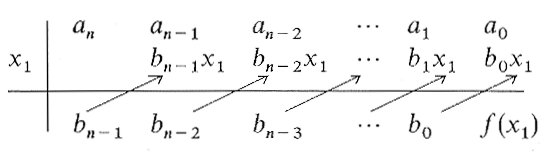
\includegraphics[width=6cm]{./bilder/hornerschema_1.png}\\
		$x_1 \Rightarrow$ Nullstelle (muss erraten werden!!)\\
		oberste Zeile = zu zerlegendes Polynom			
	\end{minipage}
	\begin{minipage}[t]{9cm}
		\textbf{Beispiel:}\\
		$f(x) = x^3-67x-126$\\
		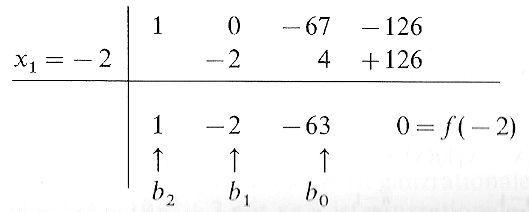
\includegraphics[width=6cm]{./bilder/hornerschema_2.png}\\
		$\Rightarrow f(x) = (x-x_1)(b_2x^2 + b_1x + b_0) = (x+2)(x^2-2x-63)$	
	\end{minipage}

\newpage

\subsection{Schrittfunktion - unit step}
	\begin{minipage}{10cm}
		$u(t) = \sigma(t) =	\begin{cases}
		  		 0 & \text{für } t < 0 \\
		  		 \frac{1}{2} \text{(praxis)}  \text{ oder undef. (math.)} & \text{für } t = 0 \\
		  		 1 & \text{für } t > 0
		  	\end{cases}
		$
		$\sigma(t) \laplace \Sigma(\omega) = \frac{1}{j\omega} + \pi\delta(\omega)$
	\end{minipage}
	\begin{minipage}{8cm}
		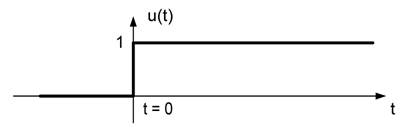
\includegraphics[width=6cm]{./bilder/unitstep.png}
	\end{minipage}

\subsection{Impulsfunktion - dirac delta function}
	\begin{minipage}{10cm}
		\begin{tabular}{l l}
		Definition & $\delta (t)=\begin{cases} 0 & t\ne 0\\\infty & t=0\end{cases}$ \\
				   & $\int\limits_{-\infty}^\infty \delta(t) \, \mathrm dt = 1 $ \\
		Zusammenhang mit der $\sigma$-Funktion & $\frac{d\sigma(t)}{dt}=\delta(t)$ \\
		Abtastung & $\int\limits_{-\infty}^{\infty} \delta(t-t_0)f(t)dt=f(t_0)$ \\
		Transformierte & $\delta(t) \laplace 1(\omega)$ \\
						& $1(t) \laplace 2\pi \cdot \delta(\omega)$ \\
		Faltung & $f(t) \ast \delta(t) = f(t)$ \\
		Ableitung & $\int\limits_{-\infty}^{\infty} \delta^{(k)}(t) \cdot f(t) dt = (-1)^k \cdot f^{(k)}(0)$ \\
		\end{tabular}
	\end{minipage}
	\begin{minipage}{8cm}
		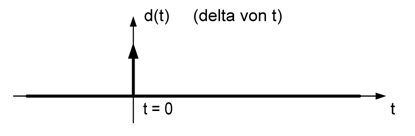
\includegraphics[width=6cm]{./bilder/diracimpulse.png}
	\end{minipage}
